\section{Апісанне арганізацыі ЭПАМ Сістэмз}

\subsection{Структура арганізацыі}
«EPAM Systems» (бел.: ЭПАМ Сістэмз) --- найбуйнейшы вытворца заказнога праграмнага забеспячэння ў Цэнтральнай і Усходняй Еўропе, рэзідэнт Парку высокіх тэхналогій Беларусі.

ЭПАМ Сістэмз аказвае кансалтынгавыя паслугі ў галіне інфармацыйных тэхналогій. 

Кампанія мае цэнтры распрацоўкі і офісы па абслугоўванні кліентаў у 20 краінах свету (дадзеныя на на 2015 г.). Колькасць супрацоўнікаў кампаніі ў Беларусі складае больш чым 2,5 тысячы чалавек. Кліенты EPAM Systems --- прадстаўнікі розных сегментаў гаспадаркі з больш чым 30 краін свету (у тым ліку з Беларусі і СНД). Сярод іх --- Microsoft, SAP, Coca-Cola, «Інтэрфакс», А1, Мазырскі нафтаперапрацоўчы завод і інш..

Паслугі:
\begin{enumerate}
    \item ІТ-кансалтынг;
    \item Распрацоўка праграмнага забеспячэння;
    \item Інтэграцыя дадаткаў;
    \item Партаванне і міграцыя дадаткаў;
    \item Тэставанне праграмнага забеспячэння;
    \item Суправаджэнне праграмнага забеспячэння;
    \item Паслугі цэнтраў кампэтэнцый.
\end{enumerate}

Сертыфікаты:
\begin{enumerate}
    \item ISAE 3402;
    \item SAS 70 Type II;
    \item CMMI Maturity Level 5;
    \item ISO 27001:2005;
    \item SEC Governed.
\end{enumerate}

На малюнку \ref{img: epam high} прадстаўлены вышэйшы ўзровень структуры арганізацыі. Можна адзначыць,
што ў ЭПАМ Сістэмз для кожнай сферы бізнеса вылучаны асобны аддзел.

\clearpage

\begin{figure}[h!]
    \centering
    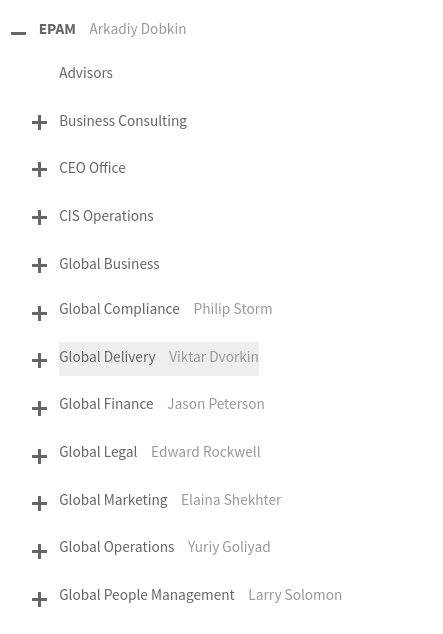
\includegraphics[width=0.4\textwidth]{epam_high.png}
    \caption{Вышэйшы ўзровень структуры ЭПАМ Сістэмз}
    \label{img: epam high} 
\end{figure}

На малюнку \ref{img: epam low} прадстаўлена структура ад вышэйшага ўзроўню да ніжэйшага, у каторым
я праходзім практыку. Як бачна з малюнка, пераддыпломная практыка праходзіла ў беларускім падраздзяленні сістэмных інжэнераў (напрамак бесперапынная дастаўка), якое 
адказвае за праекты кампаніі Liberty GLobal.

\begin{figure}[h!]
    \centering
    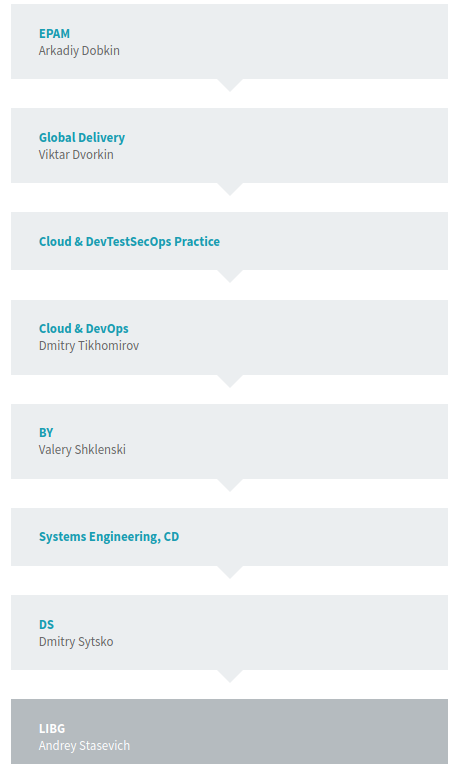
\includegraphics[width=0.3\textwidth]{epam_low.png}
    \caption{Структура падраздзялення LIBG}
    \label{img: epam low} 
\end{figure}

\subsection{Праграмнае забеспячэнне арганізацыі}

Падраздзяленне LIBG адказвае за разгортванне воблачнай інфраструктуры для IPTV сервіса кампаніі
Liberty Global.

На праекце выкарыстоўваюцца разнастайныя DevOps інструменты. Апішам некаторыя з іх.

\subsubsection{Jenkins.}

Jenkins -- найбольш папулярны праект з адкрытым кодам для аўтаматызацыі.
Дадатковае мноства плагінаў Jenkins дазваляе аўтаматызаваць
любую неабходную задачу.
Jenkins выкарыстоўваецца для зборкі праекта, запуску тэстаў,
аналізу кода і разгортвання праекта.

Асаблівасці Jenkins:
\begin{enumerate}
    \item Jenkins можа працаваць як незалежны CI сервер альбо
          як платформа бесперапыннай дастаўкі для любога праекта;
    \item наяўнасць зборак для Unix, Windows і OS X, што
          спрашчае працэс устаноўкі;
    \item наяўнасць Web-інтэрфейса для хуткай канфігурацыі сервера;
    \item разнастайныя плагіны для зборкі і кіравання зыходным кодам,
          задач адміністравання, інтэрфейсу карыстальніка.
\end{enumerate}

\subsubsection{Travis.}

Travis CI -- гэта платформа бесперапыннай інтэграцыі для аўтаматызацыі
працэсаў тэсціравання і разгортвання праграмнага забеспячэння.
Travis CI рэалізуецца ў якасці платформы, якая аб'ядноўваецца з
GitHub праектамі, што дазваляе праводзіць тэсціравання кода
ў рэальным часе.

Travis CI прадугледжвае бясплатнае выкарыстанне для адкрытых праектаў і
платная для камерцыйный праектаў.

Асаблівасці Travis CI:
\begin{enumerate}
    \item бясплатная версія для акрытых праектаў на GitHub;
    \item простая рэгістрацыя і дабаўленне праектаў;
    \item аўтаматызаваная праверка pull-запытаў;
    \item багатая падтрымка паведамленняў
          (напрыклад, e-mail, Slack, HipChat);
    \item наяўнасць API і кансольных інструментаў для
          гібкай настройкі.
\end{enumerate}

\subsubsection{GitLab CI.}

GitLab -- хуткаразвіваемая платформа для кіравання коду.
GitLab прапаноўвае ў межах адзінай панелі
інструменты для кіравання рэлізаў,
прагляду коду, бесперапыннай інтэграцыі і разгортвання.

GitLab прадугледжвае бясплатнае выкарыстанне для адкрытых праектаў і
платная для камерцыйный праектаў.

Асаблівасці GitLab CI:
\begin{enumerate}
    \item наяўнасць зборак для папулярных версій Linux;
    \item прыязны інтэрфейс карыстальніка;
    \item падрабязная дакументацыя для кожнай функцыі;
    \item магчымасць індывідуальнай настройкі тэстаў
          для кожнай галіны праекта;
    \item ручное разгортванне і лёгкай магчымасць вяртання
          на папярэднію версію.
\end{enumerate}

\subsubsection{Chef.}

Chef забяспечвае асяроддзе для аўтаматызацыі кіравання
інфраструктурай, разгортваннем, канфігурацыяй незалежна
ад памераў сеткі. Chef можна лёгка інтэгравацца ў
воблачныя сервісы, фізічныя серверы альбо гібрыдныя рашэнні.

Асаблівасці Chef:
\begin{enumerate}
    \item убудаваныя наборы інструментаў для аўтаматызацыі
          інфраструктуры як код;
    \item магчымасць кіравання як воблачнымі, так і фізічнымі
          серверамі;
    \item лёгкі перавод праграмы паміж воблачнымі серверамі.
\end{enumerate}

\subsubsection{Puppet.}

Платформа Puppet выкарыстоўваецца для кіравання канфігурацыяй для
Unix і Windows сістэмы.
Puppet -- інструмент кіравання канфігурацыяй з адкрытым кодам.
Puppet дазваляе распрацоўшчыкам дастаўляць і выкарыстоўваць
праграмнае забеспячэнне незалежна ад яго крыніцы.

GitLab прадугледжвае бясплатны тэрмін выкарыстання для азнакамлення.

Асаблівасці Puppet:
\begin{enumerate}
    \item наяўнасць гібкай настройкі Puppet-агента і кансолей, што
          дазваляе аб'ядноўваць працэсы бесперапыннай інтэграцыі;
    \item наяўнасць бясплатных модулей для хуткай распрацоўкі;
    \item прадугледжваецца сумесная работа з Git і Jenkins для
          бесперапыннай аўтаматызацыі.
\end{enumerate}

\subsubsection{Better Code Hub.}

Better Code Hub -- Web-сервіс для аналізу зыходнага кода.

Better Code Hub прадугледжвае бясплатнае выкарыстанне
для адкрытых праектаў і платная для камерцыйный праектаў.

Асаблівасці Better Code Hub:
\begin{enumerate}
    \item неадкладная зваротная сувязь на кожнае змяненне кода;
    \item інтэграцыя з GitHub;
    \item гібкая настройка прыярытэтаў дзеянняў.
\end{enumerate}

\subsubsection{Docker.}

Docker -- праграмнае забеспячэнне для аўтаматызацыі разгортвання і
кіравання праграмамі ў асяроддзі з падтрымкай кантэйнерызацыі.
Docker дазваляе ўпакаваць праграму з неабходным асяроддзем і
залежнасцямі ў кантэйнер, які можа быць перанесены на любую
Linux-сістэму.

Асаблівасці Docker:
\begin{enumerate}
    \item незалежнасць праграмы ад сістэмы, на якой выконваецца
          запуск;
    \item павялічаная бяспека сістэмы;
    \item лёгкая дастаўка праграмнага забеспячэння кліенту.
\end{enumerate}


\subsubsection{Git і GitHub.}

Git -- размеркаваная сістэма кантролю версій, якая дае магчымасць
распрацоўшчыкам адсочваць змены ў файлах і працаваць сумесна з іншымі
распрацоўшчыкамі.
GitHub -- сервіс анлайн-хостынга рэпазіторыяў, якія маюць усе функцыі
размеркаванага кантролю версій (Git) і функцыянальнасцю кіравання
зыходным кодам. GitHub дае распрацоўшчыкам магчымасць захоўваць
код анлайн, а затым узаемадзейнічаць з іншымі распрацоўшчыкамі ў
розных праектах.
Да праекта, які размешчаны на GitHub, можна атрымаць доступ пры
дапамозе інтэрфейса каманднага радку Git і Git-каманд.

Асаблівасці Git:
\begin{enumerate}
    \item рэзервнае капіраванне;
    \item простае галінаванне;
    \item высокая прадукцыйнасць.
\end{enumerate}
